\graphicspath{{./Images/Kapitel5/}}

	\section{Sensoren}
		\subsection{Allgemeines} 
		
		Abbildung \ref{fig:TS01} zeigt eine grafische Übersicht der wichtigsten Sensoren in einem Fahrzeug:
				
		\begin{figure}[h!]
			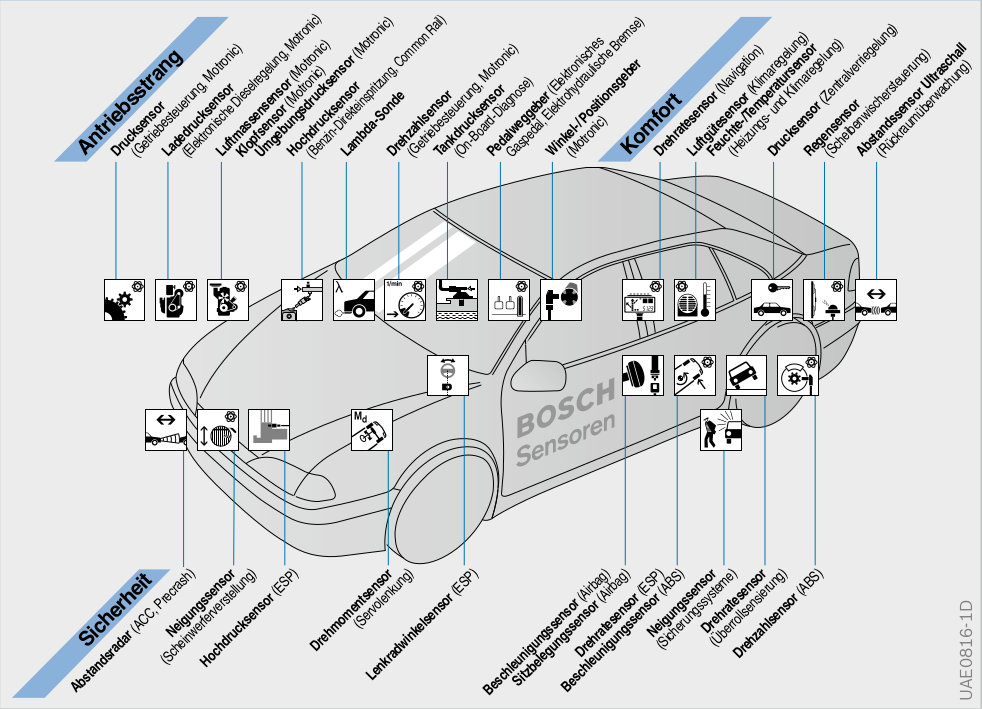
\includegraphics[width=\textwidth] {sensor_uebersicht.png}
	        \caption{Übersicht der Sensoren im Fahrzeug \cite{reif2011bosch}}
	        \label{fig:TS01}
		\end{figure}	
		
			\subsubsection{Begriffsdefinition}
		
	        Unter Sensor versteht man im allgemeinen eine
	        \begin{itemize}
	            \item Komponente
	            \item Fühler
	            \item Detektor
	            \item Aufnehmer
	        \end{itemize}
	            der eine physikalische Größe oder chemische Effekte durch messtechnische Verfahren aufnimmt und in ein analoges, elektrisches Strom- / Spannungssignal umwandelt.
	        
	        \subsubsection{Arten von Sensoren}
	
	        Grundlegend kann man zwischen mechanischen und nicht-mechanischen Sensoren unterscheiden. \\
	        \begin{itemize}
	            \item \textbf{Mechanische Sensoren}: verändern durch mechanische Einwirkungen von außen, zum Beispiel durch Kraft- oder Druckeinwirkung, ihre elektrische Eigenschaften.
	            \item \textbf{Nicht-Mechanische Sensoren}: verändern ihre Eigenschaften durch nicht-mechanische Einwirkungen, zum Beispiel chemisch durch Lichteinwirkung.
	        \end{itemize}
        
	        \begin{table}[h]
	        \begin{tabularx}{\textwidth}{l|l|l}
	
	                    \textbf{Sensorart} & \textbf{Messtechnik} & \textbf{Beispiele}\\
	                    \hline
	                    \multicolumn{3}{l}{\textbf{Mechanische Sensoren}}\\
	                    \hline
	                    Resistiv & Elektrische & Dehnungsmessstreifen \\
	                    &Widerstandsänderung& Potentiometrische Sensoren\\
	                    \hline
	                    
	                    Kapazitiv & Kapazitätsänderung & Drucksensor\\
	                    && kapazitiver Näherungsschalter \\
	                    \hline
	                    
	                    Temperatur & Kontaktthermometrie & Thermoelement\\
	                    && Widerstandsthermometer \\
	                    \hline
	                    
	                    \multicolumn{3}{l}{\textbf{Nicht-Mechanische Sensoren}}\\
	                    \hline
	                    
	                    Induktiv & Änderung der Induktion & Schwingungsaufnehmer \\
	                    && Induktivaufnehmer\\
	                    \hline
	                    
	                    Wirbelstrom & Änderung des Wirbelstroms & Induktive Initiatoren\\
	                    \hline
	                    
	                    Magnetfeld & Änderung des Magnetfelds & Hall-Generator\\
	                    && Feldplatte\\
	                    \hline
	                    
	                    Optoelektisch & Änderung der Lichtstärke & Fototransistor\\
	                    && Fotodiode\\
	                    
	
	                \end{tabularx}\\
	                \caption{Arten von Sensoren~\cite{TS_sensor_aufteilen}}
	                \label{fig:TS09}
	            \end{table}
	         	
	                	Desweiteren wird zwischen aktiven und passiven Sensoren unterschieden. 
	                	
	                	Ein aktiver Sensor ist selbst ein Spannungserzeuger und benötigt keine weitere elektrische Hilfsenergie, um betrieben zu werden. Beispiele dazu wären ein Thermoelement, Licht- oder Drucksensor.\\
	                	
	                	Passive Sensoren hingegen benötigen eine aktive Spannungsversorgung, auch Sekundärelektronik genannt, welche es erlaubt, die Messung in elektrische Signale, also in Primärelektronik, umzuwandeln. Beispiele dazu wären eine Wägezelle, Dehnungsmessstreifen, Magnetfeldsensoren.		
	                	
	\newpage                                        
	\subsection{Klassische Sensoren im Automobil} 
	       
	    Nach dieser allgemeinen Grobeinteilung von Sensoren, soll nun im Weiteren spezieller auf die Sensortechnik in Kraftfahrzeugen eingegangen werden.
	
	    Der Grund für die immer umfangreichere Sensortechnik in Automobilen liegt in der Veränderung des Automobils im Laufe der Zeit, insbesondere im Hinblick auf Fahrunterstützung und Fahrhilfssysteme.
	     	
	    Die Sensoren dienen hierbei der Eingabe,  bzw. dem Auslesen eines tatsächlichen Wertes (Ist-Wert). Diese werden einer ECU über ein Bussystem übermittelt, welches einen Abgleich des Ist-Wertes mit einem vorgegebenen Soll-Wert vornimmt und dementsprechend das Modul nachregeln und steuern kann. \\ 
	    
		Da Sensoren diversen äußeren physikalischen und/ oder chemischen 
		Einwirkungen ausgesetzt sind, müssen sie diesen entsprechend 
		gerecht werden. Aus diesem Grund gibt es verschiedene 
		Anfertigungsformen wie wasserdicht, dreck- und staubgeschützt.\\
	            
	    Ein Ausfall des Sensors kann durch folgende Ursachen hervorgerufen werden:
	
	        \begin{itemize}
	            \item Kurzschluss
	            \item Leitungsunterbrechung
	            \item Verschmutzung
	            \item Mechanische Beschädigung
	            \item nicht korrektes Anbringen des Sensors
	            \item Sensor defekt
	        \end{itemize}	
	        
	        Nach einem Ausfall kann durch gezielte Fehlersuche der Fehler analysiert werden:
	
	        \begin{itemize}
	            \item Anschlüsse prüfen
	            \item Auslesen des Fehlerspeichers
	            \item Allgemeine optische Prüfung
	            \item Säubern der Sensoren
	            \item Messungen mit einem Messinstrument vornehmen wie:
	            \begin{itemize}
	                \item Oszilloskop 
	                \item Voltmeter
	                \item Amperemeter
	                \item Ohmmeter	
	            \end{itemize}
	            
	        \end{itemize}
	
			In den nachfolgenden Beschreibungen sind einige, in Abbildung \ref{fig:TS01} dargestellte Sensoren, zusammengefasst, da die Funktionsweise mancher Sensoren sehr ähnlich sind.
			
	        \subsubsection{Temperatursensor NTC}
				Bei einem Temperatursensor handelt es sich um einen nicht-mechanischen, aktiven	Sensor, welcher die Temperatur erfasst.\\
	            Die Sensoren sind auf einen Messbereich zwischen -40$^\circ$C und +200$^\circ$C skaliert.
	            Für Temperaturen, die über diesen Bereich herausgehen, werden spezielle Hochtemperatursensoren (HTS) verwendet.
	
	            \begin{figure}[h]
				
		        	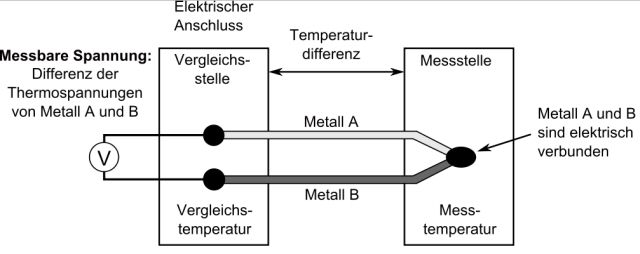
\includegraphics[width=\textwidth]{aufbau_ntc.png}
		            \caption[www.kfztech.de/kfztechnik/elo/sensoren/ntc.htm]{Aufbau NTC}
		            \label{fig:TS02}
	            
				\end{figure}
	
	            Abbildung \ref{fig:TS02} zeigt den Aufbau eines Temperatursensors.
	
	            Hierbei werden zwei unterschiedlich, elektrisch aufgeladene Metalle am Ende (der Messstelle) miteinander verbunden. Hier wird die Temperatur von dem zu messenden Element gemessen.\\
	            Die Temperaturdifferenz wird an den zwei offenen Enden mit Hilfe des Seebeck-Effekts in elektrische Spannung umgewandelt. 
	            Dann kann die Differenz der beiden Leiter verglichen werden, wobei einer der Leiter als Referenz benutzt wird (grauer Leiter).\cite{TS_temp} 
						
				NTC Sensoren werden beispielsweise in folgenden Komponenten verwendet:
				
				\begin{itemize}
					\item Katalysator
					\item Öltemperatur
					\item Klimaanlagen
					\item Kühlwassertemperatur 	
				\end{itemize}
				
	            HTS hingegen werden für
	            
				\begin{itemize}
					\item AGR
					\item Turbolader
					\item Rußfilter 
	            \end{itemize}
	            
	            eingesetzt.
	
	            \subsubsection{Induktive Sensoren}
			
	            Induktive Sensoren arbeiten nach dem Induktionsgesetz.
	            
				Hierbei erleidet der Sensor keinerlei Verschleiß, da kein direkter Kontakt zu dem zu messenden Objekt existiert.\\
				Für ein Verständnis, wo diese Sensoren welche Aufgaben im KFZ- Bereich erfüllt, reicht es nur den groben Aufbau zu kennen.\\
				Eine Spule wird von Strom durchflossen, welche daraufhin ein Magnetfeld erzeugt.\\	
	
				\begin{figure}[h]
					\centering
					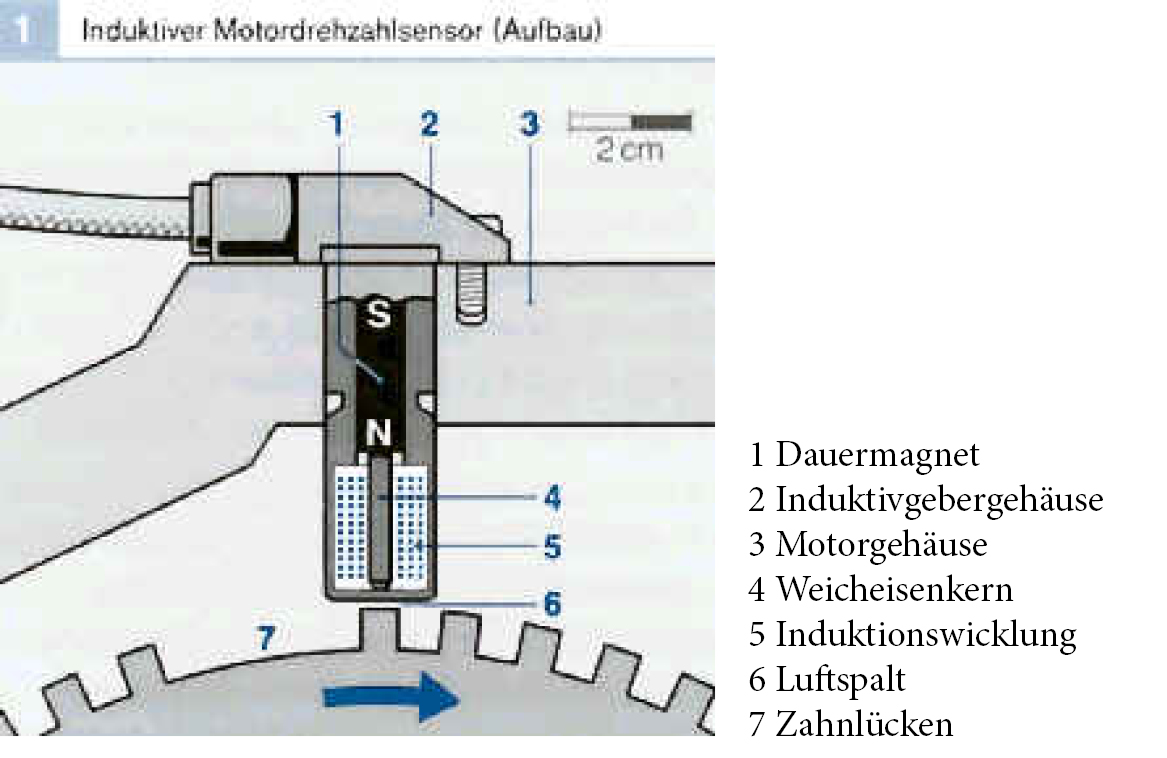
\includegraphics{Induktiv_mit_legende.jpg}
					\caption[www.kfztech.de/kfztechnik/elo/sensoren/induktivgeber.htm]{Induktiver Sensor}
					\label{fig:TS03}
				\end{figure}
				
				In Abbildung \ref{fig:TS03} ist der Sensor über einer Art Zahnrad, welches man Impulsrad nennt, angebracht.\\
	            
	            "Der magnetische Fluss durch die Spule hängt davon ab, ob dem Sensor eine Lücke oder ein Zahn gegenübersteht. Ein Zahn bündelt den Streufluss des Magneten, eine Lücke dagegen schwächt den Magnetfluss." \cite{TS_ind_funkt}  
				Die Anzahl der Änderungen/ Impulse in einer bestimmten Zeiteinheit ist ein Maß für die Drehzahl des zu messenden Objekts. Darüber hinaus kann auch die exakte Position des Moduls erkannt werden.\\					
	            
				Induktive Sensoren werden beispielsweise in folgenden Modulen verwendet:
				
				\begin{itemize}
					\item Drehzahlerfassung wie
						\begin{itemize}
							\item Kurbelwellenstellung
							\item Getriebe
						\end{itemize}	
					\item Drosselklappenstellung
					\item Lenkwinkel z.b. ESP
					\item Fahrpedalgeber
					\item Bremspedal
				\end{itemize}
			
				Allerdings kann der Ausfall eines Sensors zu erheblichen Schäden und sicherheitstechnischen Gefährdungen führen:
				\begin{itemize}
					\item Motor kann aussetzen oder gar stillstehen
					\item es wird ein Fehlercode abgespeichert
	            \end{itemize}
	           
	           
	           \subsubsection{Drehzahlsensor}
		           
		           Durch drei entsprechend angeordnete Sensoren kann die Drehrichtung des Rades erkannt werden. Ein entsprechend angeordneter Magnet (Abbildung \ref{fig:TS10}) ersetzt hierbei die Funktion der mechanischen Zahnräder.\\
		           \textbf{Aktive Sensoren}: Dieser wird bereits mit Spannung versorgt und erzeugt aus dem wechselnden Magnetfeld ein Rechtecksignal und sendet diese unverändert an ein Steuergerät.
		           
		           Dies ermöglicht ebenso eine Geschwindigkeitsmessung von 0.1km/h. Diese Werte kann man zum Beispiel für Einparksysteme oder Navigationssysteme benutzen.\cite{TS_drehzahl_sensor}
		           (Abbildung \ref{fig:TS11})
		           
		           \begin{figure}[h]
			           \begin{minipage}[b]{.4\linewidth} % [b] => Ausrichtung an \caption
			           		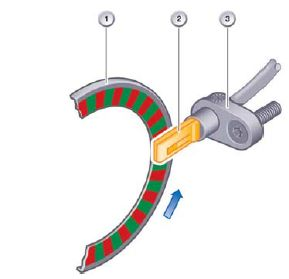
\includegraphics[width=\linewidth]{radsensor.png}
			           		\caption{Aufbau}
			           		\label{fig:TS10}
			           \end{minipage}
			           	\hspace{.1\linewidth}% Abstand zwischen Bilder
			           	\begin{minipage}[b]{.4\linewidth} % [b] => Ausrichtung an \caption
			           		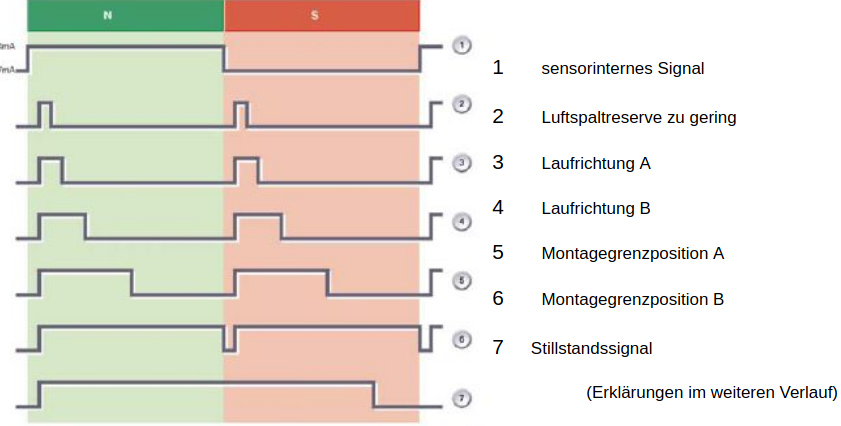
\includegraphics[width=\linewidth]{signalverlauf_hall.png}
			           		\caption[www.kfztech.de/kfztechnik/elo/sensoren/drehzahlsensor.htm]{Signalverlauf}
			           		\label{fig:TS11}
			           	\end{minipage}
		           	\end{figure}
	           
					Diese kommen beispielsweise bei:
		           	\begin{itemize}
		           		\item Getriebe und Motorik
		           		\item Navigation
		           		\item ESP
		           		\item ABS
		           	\end{itemize}
					
					zum Einsatz.	          		
	          		
	          
	           \subsubsection{Luftmassenmesser}
	           
	            Der Sensor misst im Prinzip die Luftmasse pro eingestellter Zeitspanne. Da der Massenstrom in einem bestimmten Verhältnis, meist proportional, zu dem enthaltenen Sauerstoffgehalt ist, kann dies zur Regularisierung des Verbrennprozesses im Motor beisteuern.
	           
	            \subsubsection{Ölsensor}
						
	            Dieser Sensor wird verwendet, um Informationen über den Zustand und den Füllstand des Öls zu erhalten. So kann angezeigt werden, ob und wann ein Ölwechsel notwendig ist. 
	            Das Einbringen des Ölsensors spart also Geld, schont die Umwelt und gibt Rückschlüsse auf den Zustand des Motors und es können Motorschäden verhindern.\cite{TS_oel}
	            
	            \subsubsection{Drehmomentsensor}
	            
	            Die Funktionsweise eines Drehmomentsensors kann auf zwei Arten realisiert werden:\\
	            
	            \begin{enumerate}
	                \item \textbf{Magnetoresistives Prinzip}:
	                
	                         Mittels Eingangswelle, Torsionsstab/ Drehstab (eine stabförmige Feder, welche sich in axialer Richtung drehen lässt), Antriebswelle und einem magnetoresistivem Element. \\
	                         Damit Leitungen zur Spannungsversorgung und Signalübertragung nicht beschädigt werden, sind diese in einer Vermantelung, welche auch als Wickelkassette bezeichnet wird.\\
	                         
	                         Durch das Einlenken des Fahrers wird der Torisonsstab ebenfalls verdreht. ``Diese Verdrehung ist ein Maß für das Lenkmoment.`` \cite{TS_dreh}
	
	                         Durch gezieltes Aufbringen von Widerständen können die Drehbewegungen registriert werden. Durch das Drehen, also spannen oder stauchen der Feder ( Fahrer lenkt links bzw rechts ein) verändert sich das Magnetfeld, welches wiederum den elektrischen Widerstand verändert und somit die über dem Widerstand anliegende Spannung. Diese Spannungssignale werden über die Signalleitungen an das Steuergerät übersendet, welches aus den Informationen die aufzubringende Unterstützungsmomente berechnen kann.				 
	
	                \item \textbf{Optisches Prinzip}:\\
	
	                        Vor und hinter dem Torsionsstab ist jeweils eine Scheibe angebracht, welche eine bestimmte Codierung mittels eingelassenen Löchern hat (siehe Abbildung \ref{fig:TS05}).\\
	                        Zur Bestimmung der Einlenkgeschwindigkeit wird axial und parallel zu dem Torsionsstab eine Leuchtdiode (über der ersten Scheibe) und eine Fotodiode (unter der zweiten Scheibe) angebracht. \\
	                        Die Leuchtdiode sendet gebündeltes Licht aus, welches auf der gegenüberliegenden Seite von der Fotodiode erkannt wird. Bei einfallendem Licht verändert sich der durchfließende elektrische Strom durch die Fotodiode.\\
	                        Dreht sich also die Scheibe kommt es zu einem Wechsel der Stromstärke. Diese Impulse werden an das angebundene Steuergerät gesendet, welches aus diesen empfangenden Informationen die Drehgeschwindigkeit berechnen kann.\\
	                        
	                        \begin{figure}[h]
	                            \centering
	                            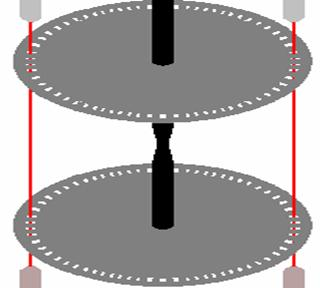
\includegraphics{photoelektrisch.png}
	                             \caption[www.kfztech.de/kfztechnik/fahrwerk/lenkung/photoelektrisch.jpg]{Photooptisches Prinzip}
	                             \label{fig:TS05}
	                        \end{figure}	
	            \end{enumerate}
				
				Einsatzgebiete könnten zum Beispiel der Lenkdrehmomentsensor im Bereich der Servolenkung sein: \\
				``Um die Funktion des Servomoduls umsetzen zu können, benötigt das Steuergerät exakte Informationen über die vom Fahrer eingegebene Lenkbefehle. Um diese Eingabe richtig erfassen zu können, wurde ein Sensor konstruiert, welcher [...] die erforderlichen Daten wie Drehwinkel, Drehrichtung und Drehmoment elektronisch erfassen.[...] ``  \cite{TS_dreh} kann und an das Steuergerät sendet.\\
				
				
	            \subsubsection{Regensensor}
	
	                Dieser nicht-mechanische Sensor ``[...] registriert Wassertropfen auf der Windschutzscheibe durch opto-elektrisches Verfahren`` \cite{TS_regen}
	                
	                Der Regensensor befindet sich innerhalb des Wischbereichs des Scheibenwischers.                
					In dem Sensor befindet sich eine Leuchtdiode und eine Fotodiode, welche in einem bestimmten Abstand voneinander angebracht sind. Die Leuchtdiode sendet ein Infrarotlicht aus. Dieses Lichtbündel wird bei trockener Windschutzscheibe an der äußeren Scheibe reflektiert und nahezu mit voller Lichtstärke von dem Sensor aufgenommen. In der Physik spricht man hier von einer Totalreflexion.\\
					Befinden sich nun Wassertropfen in dem Bereich des Sensors auf der Frontscheibe wird das ausgesendete Lichtbündel nicht komplett reflektiert, sondern ein Teil des Lichtes wird gebrochen und durch den Tropfen gestreut. Das Resultat daraus ist, dass der ausgesendete Lichtstrahl nur noch mit einem Bruchteil der ursprünglichen Stärke den Sensor erreicht.\\
					Aus diesen Daten errechnet die dort darin befindliche Elektronik die Stärke des Niederschlages, gibt diese an ein Steuergerät weiter, welches wiederum die Scheibenwischer ansteuert. Somit bleibt die Oberfläche des Sensors immer tropfenfrei und es wird ein optimales Messergebnis erreicht. ( Abbildung 8)
					
					\begin{figure}[h]
						\centering
						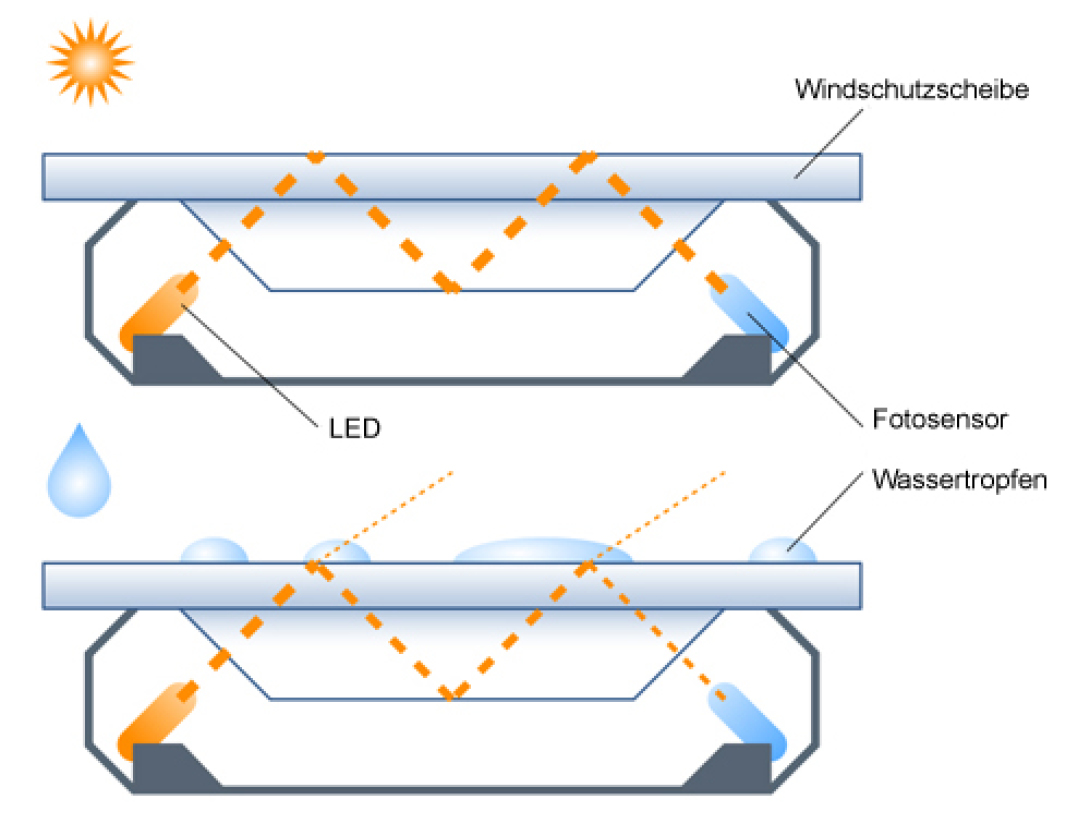
\includegraphics{regensensor2.jpg}
	                    \caption[archiv.langzeittest.de/volvo-s40/intern/grafik/cb-regensensor-prinzip.jpg] {Prinzip eines Regensensors}
	                    \label{fig:TS06}
	                \end{figure}
	                
	            \subsubsection{Seitenwandtorsionssensor}
	
					Elektronische Regelsysteme wie ABS oder ESP benötigen sämtliche Informationen über das Zusammenspiel zwischen Fahrzeug und dem Fahruntergrund und den daraus entstehenden Kräften. Um die einzelnen Sekundärgrößen wie Motorleistung, Bremsdruck, Radgeschwindigkeit und Fahrzeugbeschleunigung zur Berechnung nicht mehr benutzen zu müssen, wurde von Continental ein Sensorsystem entwickelt, welches das Rad als Sensor fungieren lässt, das sogenannte SWT-System. 
					
					\begin{figure}[h]
						\centering
						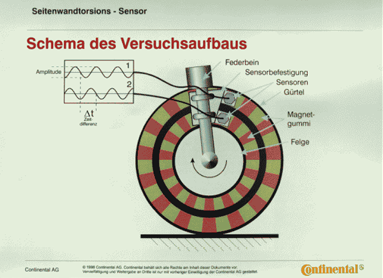
\includegraphics[width=\linewidth]{swt1.png}
	                    \caption[www.kfztech.de/kfztechnik/sicherheit/swt/swt1.gif]{Reifen als Sensor}
	                    \label{fig:TS07}
					\end{figure}
				
	                Der Reifen besteht aus Magnetgummi und Magnetfeldsensoren, sowie einem Signalaufbereitungssystem und einer zentralen Recheneinheit.
						
	                Die Messung findet mittels der Verformung des Reifens statt, die entsteht wenn der Reifen bei Kurvenfahrten durch die einwirkenden Querkräfte temporär aus der Form gebracht wird. 
	                
	                Hierfür werden zwei Sensoren am Fahrwerk angebracht, wobei einer der beiden auf der Höhe der Felge ist und der andere nahe am Scheitelpunkt des Reifens angebracht wird. Darüber hinaus ist die Reifenseitenwand magnetisch, um ein Messergebnis erzielen zu können.\\
	                In der obrigen Abbildung erkennen wir ein Muster auf dem Reifen. Dies ist darauf zurückzuführen, dass ein Magnetpulver in die Reifenseitenwand eingemischt wird. Dieses Gemisch wird über den gesamten Umfang des Reifens gestrichen und somit erhält man eine alterniernde Nord- und Südpole, was durch die Streifen visualisiert wird.
	                
	                Solange auf den Reifen keine Längskräfte wirken, ``[]...] erfolgt der Wechsel zwischen den Magnetpolen an beiden Sensoren gleichzeitig, die Zeitdifferenz zwischen den Signalen beider Sensoren ist Null`` \cite{TS_swt} \\	
	                Beschleunigt oder verzögert der Fahrer das Fahrzeug, überschreiten die Grenzen der Magnete zu unterschiedlichen Zeiten die Sensoren, somit ist eine Zeitdifferenz zu messen. 
	                Diese gemessene Zeitdifferenz wird an ein eingebautes Steuergerät gesendet, welche die Fahrassistenzsysteme wie ASR und ABS anspricht und dementsprechend der derzeitigen Fahrsituation anpasst.\\
	                
					Während einer Kurvenfahrt kann der Abstand zwischen der Reifenseitenwand und dem Sensor gemessen werden, da sich dieser mechanisch gesehen verkürzt bzw. vergrößert wird und sich somit die Stärke des Magnetfelds ändert.\\
	                Mit Hilfe dieser gemessenen Werten können Hilfssysteme wie ABS und ESP entsprechend angesteuert werden. Dies sorgt für ein sichereres Fahren da die Ansteuerung optimiert werden kann. 
	                
	                In der Praxis bedeutet dies, dass der Fahrer einen kürzeren Bremsweg und eine bessere Kontrolle über das Fahrzeug auf kurvenreichen und schweren Strecken hat.
	
	                \subsubsection{Reifensensor}
	
	                Ein in den Reifenprofil eingebetteter Chip überträgt hochfrequent die Signale an eine im Radkasten befindliche Antenne. 
	                Ändert sich der Zustand der Straße verändert der Sensor das Signal. Dies geschieht pro Sekunde mehrere Male. 
	                Darüberhinaus kontrolliert der Sensor permanent den Reifendruck. Mit diesen Informationen kann nicht nur die Lebensdauer des Reifens, sondern auch die Sicherheit erhöht werden, 
	                da sich gezielt ABS und ESP einschalten.\\ 
				
	                \subsubsection{Reifendrucküberwachungssystem}
	                Reifendrucküberwachungssysteme (RDKS) werden eingesetzt, um die Lebensdauer des Reifens zu erhöhen. Seit 1. November 2014 sind die Reifen- und Autohersteller verpflichtet, ein RKDS zu implementieren.
	                Hierbei wird jeder Reifen mit einem Sensor ausgestattet, damit der Fahrer Luftverlust oder gar einen Plattfuß bemerken kann.
	                
	                Prinzipiell gibt es RDKS in aktiver und passiver Variante. In Tabelle \ref{fig:TS08} werden diese in Funktionsweise mit ihren jeweiligen
	                Vor- und Nachteilen gegenübergestellt.
	
	                \begin{table}
	                    \begin{tabularx}{\textwidth} {l|l}
	                        
	                        
	                        \multicolumn{2}{c}{\textbf{Passives Reifendrucküberwachungssystem}}\\
	                        \hline
	                        \textbf{Erklärung:} & Platter Reifen hat einen kleineren Abrollumfang \\ & und dreht sich schneller.\\ & ABS Sensoren messen dies und das Steuergerät erkennt dies\\
	                        \hline
	                        \textbf{Vorteil:} & kostengünstig, in Kombination mit Runflat Tyres eine \\ & optimale Lösung, da nur eine geänderte Software \\ & und Kontrolle erforderlich sind.\\
	                        \hline
	                        \textbf{Nachteil:} & schleichender Luftverlust der Räder an einer Achse \\ &  wird nicht erkannt. Nur Differenzen größer 0.5 Bar werden \\ & während der Fahrt erkannt. Höherer Spritverbrauch durch \\ & zu niedrigen Luftdruck.\\
	                        \multicolumn{2}{c}{\textbf{Aktives Reifendrucküberwachungssystem}}\\
	                        \hline
	                        \textbf{Erklärung:} & Jeder Reifen besitzt eigenen Sensor und sendet Informationen \\ & über Druck und Temperatur per Funk an Steuergerät.\\
	                        \hline
	                        \textbf{Vorteil:} & Exakte Messung, ab einer Differenz von 0.2 Bar wird ein \\ & Alarm ausgelöst. Reserverad wird mit überwacht.\\
	                        \hline
	                        \textbf{Nachteil:}  & Teuer für Reifenmontage, da Reifen kodiert werden müssen\\ & und der Reifenwechsel aufwendig wird.\\
	
	                    \end{tabularx}
	                    \caption{Aktive und Passive Reifendrucküberwachungssysteme \cite{TS_rdks}}
	                    \label{fig:TS08}
	
	                \end{table}
	
	                
	                Die Reifenelektronik sitzt auf der Innenseite des Reifen und misst in kurzen definierten Zeitabständen Reifendruck und Temperatur. 
	                Jeder Sensor ist mit einer eigenen ID- Nummer ausgestattet. Per Funk werden an die eigene Empfangsstation Datenpakete geschickt, welche die ID, sowie Druck und Temperatur des Reifens beinhalten.
	
	                Dieses Empfangsgerät sendet die empfangenen Daten kabelgebunden weiter an das Steuergerät. Dieses wertet die Daten aus und sendet bei Bedarf, sprich Unter- oder Überschreitung der Sollwerte, eine Meldung an die Kontrollanzeige.
					
	                \subsubsection{Hallsensor}
	
					Hallsensoren werden eingesetzt in: 
					\begin{itemize}
						\item Zündanlage
						\item Getriebeausgabedrehzahl
						\item Radlöseerkennung/- warnung (Audi)
						\item aktiver Drehzahlsensor in ABS- Bremsanlagen
						\item Nockenwelle (Koordination von Eispritzungsbeginnberechnung oder Pumpe-Düse, sowie Klopfregelung)
					\end{itemize}
					
	                Am Beispiel des Nockenwellensensors wird im Folgenden die Funktion des Sensors beschrieben.
	                
	                Die Nockenwelle bringt einen aus ferromagnetischem Material angefertigten Rotor zum Drehen. Zwischen Rotor und einem Dauermagnet befindet sich der Sensor.
	                Durch den Dauermagneten wird ein Magnetfeld erzeugt, welches den Sensor senkrecht durchfließt. Passiert ein metallischer Gegenstand, beispielsweise ein Zahn der Nockenwelle, verändert dieser das Magnetfeld, welches den Sensor durchfließt.
					Elektronen werden senkrecht zum Magnetfeld stärker abgelenkt, wobei eine Hall-Spannung von mehreren Millivolt erzeugt. Eine integrierte Auswerteelektronik bereitet das Signal auf und leitet es an in Form eines Rechtecksignals an das Steuergerät geleitet. \cite{TS_hall}
	
					\begin{figure}[h]
						\centering
						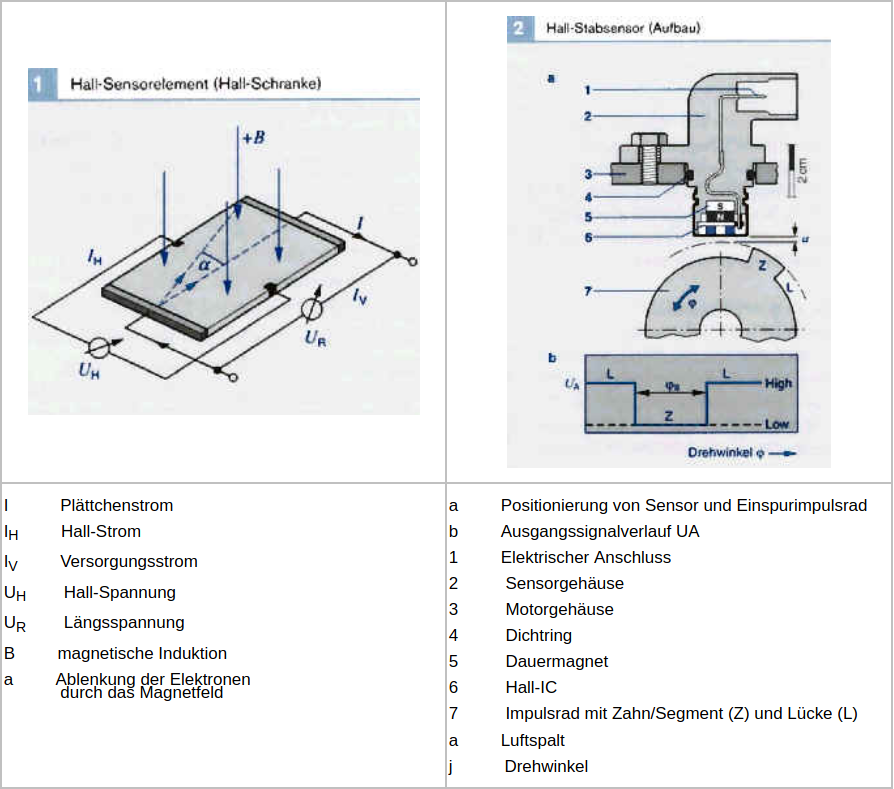
\includegraphics[width=\textwidth]{hall.png}
						\caption[www.kfztech.de/kfztechnik/elo/sensoren/hallsensor.htm]{Aufbau eines Hall-Sensors}
	                \end{figure}
	                
	                
	
				\subsubsection{Airbagsensor}
	
	                 Für das Auslösen des Airbags werden mehrere Frontsensoren verwendet, welche an diversen Stellen im Auto angebracht sind. Die Beschleunigungssensoren messen einwirkende Kräfte und geben ein Signal an das Steuergerät.
	                 Damit der Airbag nicht fälschlicherweise geöffnet wird, muss ein Sicherheitssensor innerhalb des Steuergerätes dies bestätigen. 
	                 
	                 ``Durch das genau Erfassen der Unfallschwere wird die Auslösung der Airbags und der Gurtstraffer aktiviert.`` \cite{TS_airbag}\\
	                 Faktoren sind: 
	                 
	                 \begin{itemize}
	                     \item Aufprallstärke
	                     \item Sicherheitsgurte angelegt
	                     \item Sitzposition des Fahrers und Beifahrers
	                 \end{itemize}
	             
	             
	             \subsubsection{Positionssensoren}
	
	                 Diese Sensoren sind an diversen relevanten Stellen des Automobils befestigt. Sie geben Aufschluss über Gegenstände in unmittelbarer Nähe des Fahrzeug.
	
	                 Um diese erkennen zu können wird ein Ultraschallsensor eingesetzt, welcher ein Signal aussendet. Falls ein Gegenstand in der Nähe ist, reflektiert dieser die Schallwellen und ein Ultraschallempfänger empfängt diese. 
	                 Durch die Zeitdifferenz des ausgesendeten und des erhaltenen Signals kann die Entfernung errechnet werden. Kommt das Objekt näher, so verkürzt sich der Abstand und somit auch die Zeit des Eintreffen des Schalls.
	
	                 Der Sensor sendet zu einen die Zeit, wann dieser die Ultraschallwellen gesendet hat sowie die reflektierten Signale. Aus dieser Differenz kann  der Abstand zwischen Auto und Gegenstand errechnet werden. 
	                 Nähert sich das Auto einem Objekt, so verkürzt sich die Zeit zwischen den austretenden und empfangenen Schallwellen. Bei dem kleinsten zulässigen Abstand meldet das Steuergerät dies der Kontrolleinheit und der Fahrer wird informiert.
	
	                 Falls sich kein Objekt in der Nähe befindet wird auch kein Signal reflektiert und somit erkennt das Steuergerät, dass keine Kollision stattfinden kann.
	
	                \subsection{Smarte Sensoren} 
	                 Unter smarten Sensoren versteht man Sensoren, die über eine integrierte Recheneinheit und -logik verfügen.
	                 
	                 Dadurch können diese Sensoren neben dem reinen Messen die eingelesenen Daten direkt verarbeiten und in diesem Zustand dem Steuergerät überreichen. 
	                 
	                 Dies hat den Vorteil, dass das Steuergerät keine überflüssigen Rechenschritte abarbeiten muss und somit mehr Rechenleistung für die Reaktion auf besondere Ereignisse hat.
	
	                 Smarte Sensoren können beispielsweise bei Feldbussystemen wie LIN, CAN, Flexray eingesetzt werden.		
	             	             
				 \newpage
				 
	             \subsection{Zukunftsvisionen} 
	                  Durch das Weiterentwickeln der Sensortechnik können beispielsweise Unfälle vermieden werden, da der Sensor eine deutlich schnellere Reaktionszeit aufweist als ein Mensch.
	                  Ein Beispiel wäre, das bestehende Positionssensorsystem durch eine neue Art der Messung zu ersetzen. Hierbei werden die Ultraschallsensoren 
	                  durch sogenannte Radarkameras ersetzt, welche einen deutlich weiteren Radius abdecken können, als die bisher herkömmlichen Sensoren.
	                  
					  \begin{figure}[h!]
						\centering
	                      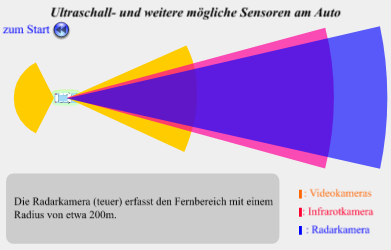
\includegraphics[width=0.7\textwidth] {radarsensor.png}
	                      \caption[www.leifiphysik.de/akustik/schallgeschwindigkeit/ausblick/\\ultraschall-beim-auto]{Unterschied: Video-, Infrarot- und Radarkamera}
	                      \label{fig:TS12}
	                  \end{figure}
	     
	                     In Abbildung \ref{fig:TS12} kann man deutlich den Unterschied in der Reichweite der verschiedenen Sensoren sehen.\\
	                     
	                     Neben diesem Effekt kann durch neue entwickelten Sensoren beispielsweise der Spritverbrauch und somit den Ausstoß an $CO_2$ verringert werden.\\
	                     Auch im Hinblick auf Elektromobilität wird es neue Sensoren geben, welche zur Überwachung der Batterie eingesetzt werden.